\chapter{Requirements and Analysis}\label{chapter3}
% This should state, in a more detailed way, the objectives of the project by requirement and the analysis should break the problem down into manageable steps. There may be more than one suitable approach; the analysis may cover more of the area than is finally implemented. Testing and evaluation should be given due consideration. It is important that you state how you will evaluate your work. For a design project it is appropriate to consider testing at the same time as specification.

This chapter will speak about solution requirements, objectives and data. In the first section, a basic idea of the aim of the solution will be discussed. The requirements will follow giving more details about the data and predictive requirements for the task. The analysis sections will speak about statistics on data and draw some broad  conclusions about what to expect, while the final section will speak about how to approach creating a solution in manageable, modular steps.

\section{Aims and Objectives}

The main goal is to create a system which will predict MWE and Supersense tags as outlined in the original \dimsum task \cite{Schneider2016}. The solution should include a sensible baseline and a system which outperforms the baseline. A sensible solution can be quantified as a system which performs within the results for the original task with an F1-Score of 27-57\%. Therefore the requirements section will speak about the baseline system and the final system within this framework. 

\section{Requirements}

The original SemEval Task 10 \dimsum defines requirements for the data and output of the system. Certain aspects of the requirements are previously defined and will be mentioned briefly here. Additional requirements were self-imposed due to constraints or deliberate choices. All will be discussed in the following sections.

\subsection{Data}
The data requirements are fairly well defined in the \dimsum task. Additional information about the data and its usage can be seen in the appendix \ref{appendixdata}. Sentences are provided in a CoNLL style file separated by newlines which contain nine columns as seen in Figure \ref{fig:dimsumcolumns}.

\begin{figure}[H]
\centering
\begin{framed}
  \centering
  \begin{ttfamily}
    \begin{enumerate}
      \setlength{\itemsep}{0pt}
      \setlength{\parskip}{0pt}
    \item token offset
    \item word
    \item lowercase lemma
    \item POS
    \item MWE tag
    \item offset of parent token
    \item strength level encoded (unused)
    \item supersense label, if applicable
    \item sentence ID
    \end{enumerate}
  \end{ttfamily}
\end{framed}
\caption{Sentence columns for \dimsum data}
\label{fig:dimsumcolumns}
\end{figure}

There are no constraints on types of systems such as rule based vs. data driven methodologies therefore any column can be used for training. The final results must predict labels in columns 5 and 8. Column number 6 must also be filled in but is deterministically defined by the prediction of the MWE labels in column 5. The labelled training files provided for the \dimsum task in \cite{dimsum16webdata} contain sentences with the columns identical to Figure \ref{fig:dimsumcolumns} with ``\texttt{blind}'' testing file counterparts which contain blank or obfuscated labels. An example sentence can be seen in Figure \ref{tab:dimsumsentence} below, taken from \texttt{dimsum16.train}, the main training data file.

\begin{table}[!htbp]
\small
\begin{framed}
  \centering
  \begin{ttfamily}
  \begin{tabular}{lllllllll}
    1 & So & so & ADV & O & 0 &  &  & ewtb.r.328828.6\\
    2 & what & what & PRON & O & 0 &  &  & ewtb.r.328828.6\\
    3 & was & be & VERB & O & 0 &  & v.stative & ewtb.r.328828.6\\
    4 & the & the & DET & B & 0 &  & n.communication & ewtb.r.328828.6\\
    5 & point & point & NOUN & I & 4 &  &  & ewtb.r.328828.6\\
    6 & of & of & ADP & O & 0 &  &  & ewtb.r.328828.6\\
    7 & the & the & DET & O & 0 &  &  & ewtb.r.328828.6\\
    8 & appointment & appointment & NOUN & O & 0 &  & n.event & ewtb.r.328828.6\\
    9 & !?! & !?! & PUNCT & O & 0 &  &  & ewtb.r.328828.6\\
  \end{tabular}
  \end{ttfamily}
  \caption{Example sentence in \dimsum training file dimsum16.train}
  \label{tab:dimsumsentence}
\end{framed}
\end{table}

All predictions must be made in the same order as the \texttt{blind} test file with the appropriate columns filled in (5,6,8). Column 9 is just for cross referencing where the sentence was retrieved from by using an unambiguous ID. In the \texttt{blind} test files it is usually filled in with an obfuscated form of the sentence ID. It is not needed for the final prediction and can be left untouched. 

Any pre or post-processing is acceptable just as long as the first 4 columns can be recreated or inferred from the original test sentence.

The data given for the \dimsum task contains an evaluation script called \texttt{dimsumeval.py}. In order to compare the results in a meaningful way, all evaluation must use this script in conjunction with the data files provided for the task. This will be spoken about in more detail in the analysis section that follows.

Any additional details on how the data was obtained and annotated can be viewed in the paper \cite{Schneider2015}.

Finally, any solution should generalise to unseen data, using labels defined in the dataset itself. 

\subsection{Prediction}
This section speaks about the requirements for the prediction of the MWEs and supersenses as well as data sparsity related issues.

\subsubsection{Multiword Expressions}
MWEs can take multiple forms in the \dimsum data. They are categorised as contiguous or gappy constructions, essentially forms of weak and strong MWEs. Due to this, the data uses a modified \texttt{BIO} style annotation with additional lowercase forms to capture ``gappy'' constructions, making possible MWE tags \texttt{BbIiOo}. The tag scheme follows the predictable scheme of {\bf B}eginning, {\bf I}nside, {\bf O}utside with the corresponding lowercase forms to capture the embedded constructions in gappy MWEs. In complete contrast to Named Entity Recognition tasks, gappy constructions {\it can} exist within the \dimsum MWE labels, which capture a wider degree of flexibility inherent in natural language. This makes the task more complex but more realistic.

\begin{table}[!htbp]
\small
\begin{framed}
  \centering
  \begin{ttfamily}
  \begin{tabular}{llllllllllll}
    I & have & a & bit & of & experience & watching & the & usual & assembly & line \\
    PRON & VERB & DET & NOUN & ADP & NOUN & VERB & DET & ADJ & NOUN & NOUN \\
    O & B & b & i & o & I & O & O & O & B & I \\
    \ & \ & \multicolumn{3}{c}{$\underbrace{\hspace{2.5cm}}$} & & & & & & \\ 
    \ & \ & \multicolumn{3}{c}{Embedded MWE} & & & & & & \\ 
    \ & \multicolumn{5}{l}{$\underbrace{\hspace{5.5cm}}$} & & & & & \\ 
    \ & \multicolumn{5}{c}{Gappy MWE} & & & & & \\ 
  \end{tabular}
  \end{ttfamily}
  \caption{Example ``gappy'' construction in training data}
  \label{tab:gappysentence}
\end{framed}
\end{table}

The difficulty in predicting such constructions requires a recognition of contiguous {\it and} gappy constructions. This is how the \dimsum task is unique from other Named Entity Recognition systems. Creating a generalisable solution is important for capturing these differences. 

\subsubsection{Supersenses}

All available top level Supersenses are represented in the training data as can be seen in \ref{tab:wordnetsupersenses}. There are 26 \texttt{NOUN} heads and 15 \texttt{VERB} heads, this means that there is a possible 41 supersense tags to be considered. The prediction of supersenses is not limited to MWEs and can be assigned to any single word which might carry semantic content. Assigning a correct supersense tag therefore depends on both cases. If a supersense is assigned to a word, it will appear in it's appropriate column in the training data for that specific word, whereas a MWE that contains a supersense tag must be assigned to it's head which are the tags \texttt{Bb} respectively. 

For example, as seen in Figure \ref{tab:dimsumsentence}, line 3 has the tag \texttt{v.stative} assigned to the word \texttt{was}, whereas line 4 has the tag \texttt{n.communication} assigned to it with the following line 5 being empty as the semantic supersense has already been assigned to the previous token. 

\begin{table}[!htbp]
\small
\begin{framed}
  \centering
  \begin{ttfamily}
    \begin{minipage}{.5\textwidth}
      \centering
      \begin{tabular}{ll}
        \multicolumn{2}{c}{Correctly Assigned Supersense}\\
        \hline
        Sihuan  & Pharmaceutical \\
        PROPN   & NOUN \\
        B       & I \\
        n.group &\\
      \end{tabular}
    \end{minipage}\hfill
    \begin{minipage}{.5\textwidth}
      \centering
      \begin{tabular}{ll}
        \multicolumn{2}{c}{Incorrectly Assigned Supersense}\\
        \hline
        Sihuan  & Pharmaceutical \\
        PROPN   & NOUN \\
        B       & I \\
        \ & n.group\\
      \end{tabular}
    \end{minipage}\hfill
  \end{ttfamily}
  \caption{Example correct/incorrect MWE supersense tagging}
  \label{tab:supersensetagging}
\end{framed}
\end{table}

As seen in the previous example in Table \ref{tab:supersensetagging}, the first example has only one assigned supersense to the head with the \texttt{B} MWE tag. The incorrect example shows the supersense assigned to the \texttt{I} MWE tag which does not follow the constraints.

These constraints must be maintained or the semantic supersense tags predicted will be considered incorrect and evaluation will not work correctly. That being said, all solutions must stick to this constraint and assign a single supersense per word or per MWE head for all words contained within the MWE.

The idea for these constraints is to assigned semantic information to single semantic units. Since MWEs are considered to be a single semantic unit, irrespective of their construction, only a single semantic sense should be assigned. 

A solution to the \dimsum task must take these constraints into account when predicting supersenses.

\section{Analysis}
In this section, an analysis of the data and project will be explained, with an attempt to clarify data and draw initial conclusions. 

Initially, looking at some statistics related to the training data was the first was step taken to give us insight on task. The following is stated in the \texttt{TAGSET.md} file in the \dimsum data. 

\begin{table}[H]
\centering
\begin{tabular}{|cccccc|}
\hline
      & \multicolumn{2}{c}{Not inside gap} & \multicolumn{2}{c}{Inside gap} & \\
\hline
      & Count & Token & Count & Token & \\
\hline
\hline
      & 63264 & O & 675 & o & \\
      &  4208 & B & 24  & b & \\ 
      &  5623 & I & 32  & i & \\
\hline
\hline
      &       &   &     &   & All tokens\\
\hline
Total & 73095 &   & 731 &   & 73826\\
\hline
\end{tabular}
\caption{Token-level MWE-positional flags with frequency counts}
\label{tab:mwetokencounts}
\end{table}

Supersense count statistics shed light on the frequency of noun or verb types as seen in Table \ref{tab:ssnvcounts}.

\begin{table}[H]
\centering
\begin{tabular}{cc}
noun  & verb\\
\hline
12591 & 9863\\
\end{tabular}
\caption{Supersense frequency counts in \dimsum training data}
\label{tab:ssnvcounts}
\end{table}

Finally, the top counts of each supersense are demonstrative relative clues for semantic nature of MWEs.

\begin{table}[H]
\centering
\begin{tabular}{lcc}
n.person & v.stative\\
\hline
1867     & 3357\\
\end{tabular}
\label{tab:topssnvcounts}
\caption{Top supersense frequency counts per category}
\end{table}

From the statistics in the original \texttt{TAGSET.md} file we can state the following.

{\bf The majority of:}
\begin{enumerate}
  \setlength{\itemsep}{0pt}
  \setlength{\parskip}{0pt}
\item MWE Tokens are \texttt{O}
\item MWEs are not gappy
\item Supersenses are noun types
\item Noun supersenses are n.person
\item Verb supersenses are v.stative
\end{enumerate}

Since the majority of MWE tokens are \texttt{O}, we know that the majority of words are {\bf O}utside an MWE. Also, most MWEs are strong or continuous as only a small minority are the gap internal counterpart labels. This inherently means most MWEs are not weak, so our system should at least be able to recognise continuous MWEs well as well at use the outside tag in a correct way. It could potentially use it for unseen data considering it to be the safest conclusion to make as it is the most common label on a per token basis. This is in fact the case as described in Chapter \ref{chapter4}, the default label is \texttt{O} for unseen data.

An additional script was written to read the data files provided with the task which sheds additional light on the relationship of supersenses for MWEs.

\begin{figure}[H]
\centering
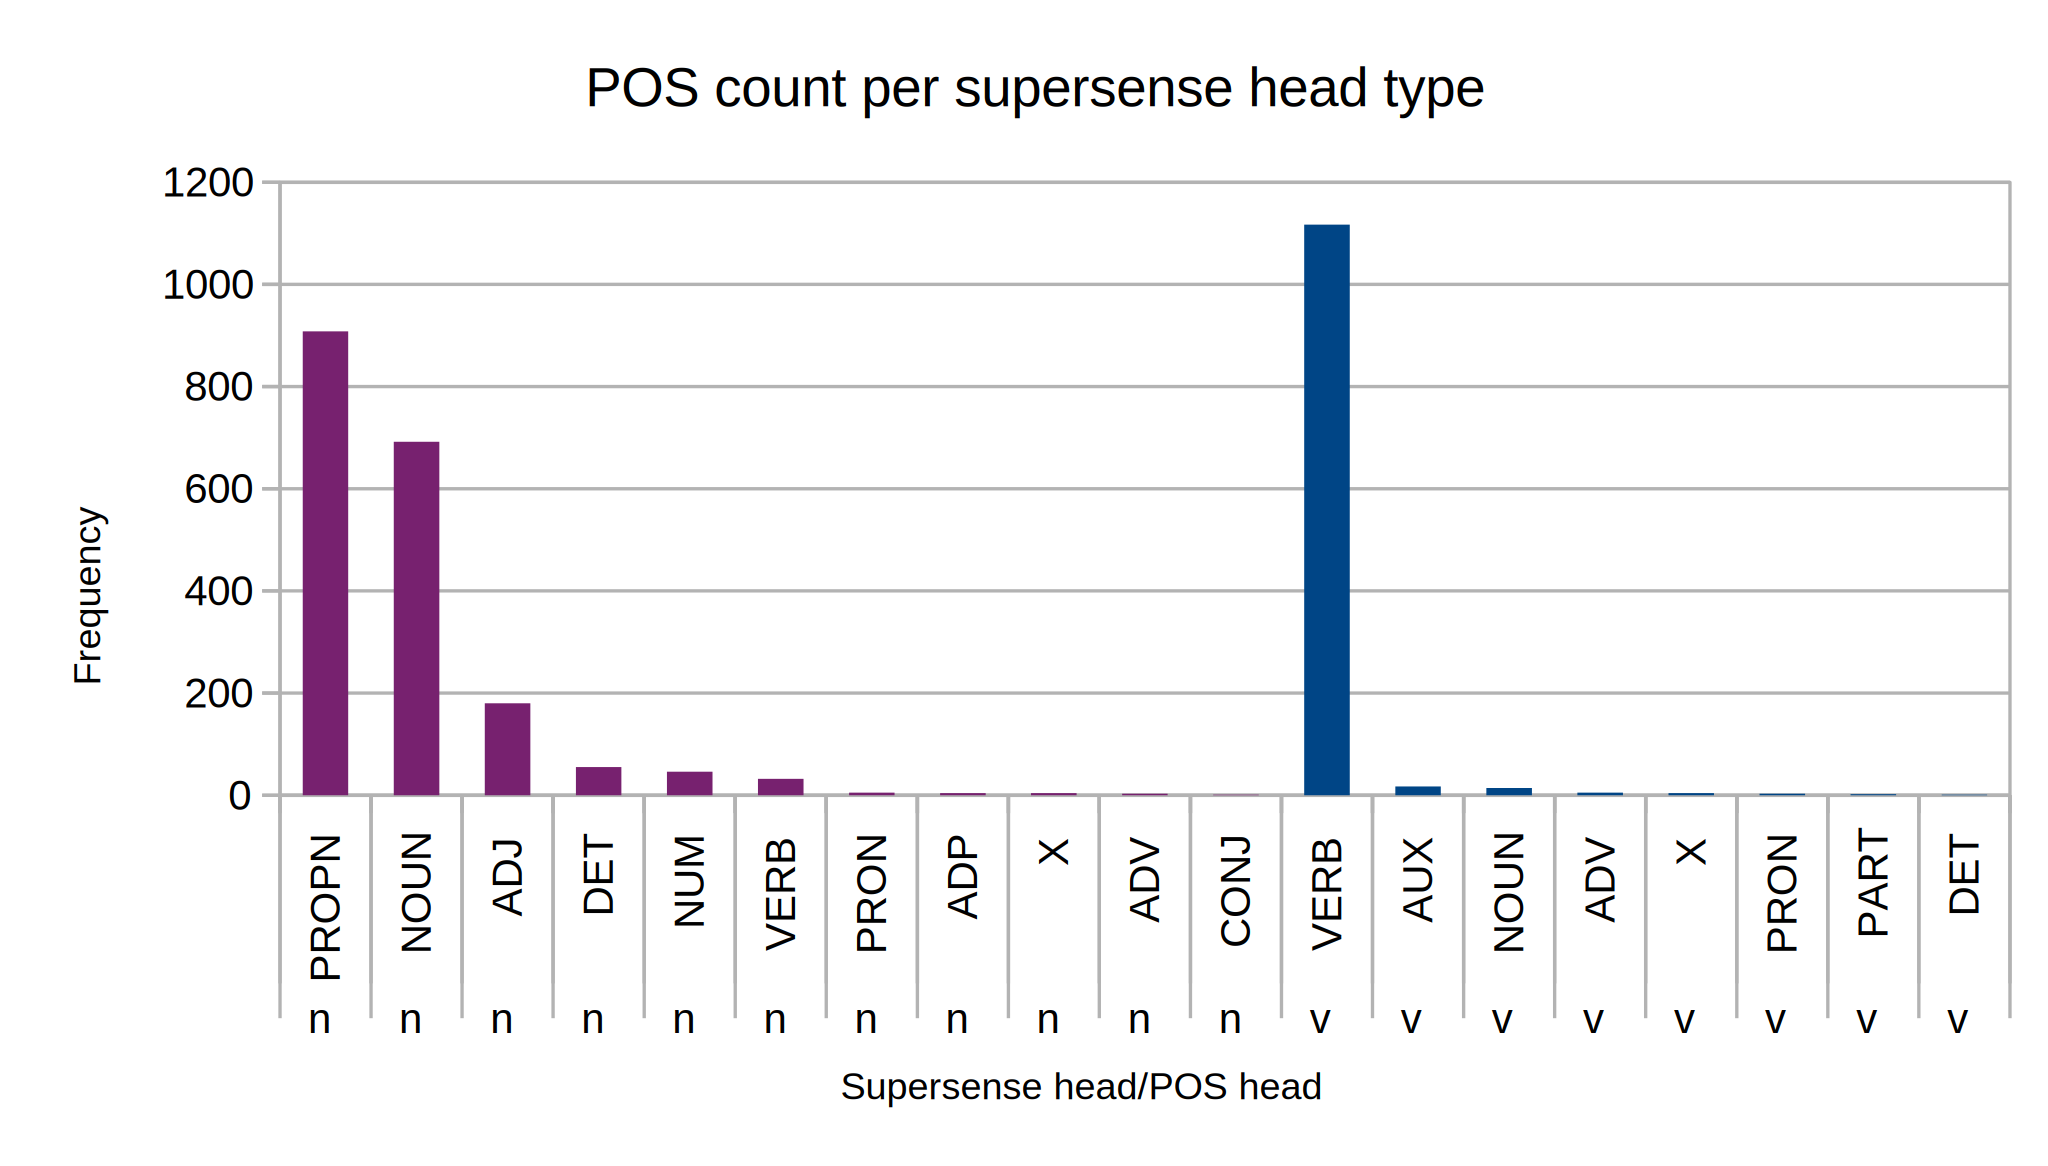
\includegraphics[width=0.8\textwidth]{images/pos_ss_freq.png}
\caption{POS frequency count per Supersense Head type}
\label{fig:posfreqperss}
\end{figure}

Figure \ref{fig:posfreqperss} shows the quantity of times a POS tag is seen for a given super sense head type (either n. or v.). This shows that the majority of times a noun supersense is tagged, its corresponding head is a proper noun. This in conjunction with the fact that most supersenses are tagged \texttt{n.person} would lead us to believe many noun headed supersenses are in fact named entities. Almost all verb headed supersenses have a POS tag of VERB which is not so informative. What is informative is the lower counts which show that many verb headed supersenses do not have a POS tag of VERB. 

These statistics give us information about what single types of supersense or MWE tags are occurring in the data but are uninformative in regards to context. Contextual clues will give us the information to create a robust solution. 

\section{Modularity and Procedure}

This final section will attempt to use the previous information in this chapter to outline a meaningful approach to modularising data and results into different stages. These stages will help draw conclusions about the systems, their predictive capacity and robustness of solution.

\subsection{Baseline system}
The baseline system should be a full solution to the task which uses a sensible albeit simple approach. The original paper \cite{Schneider2016} defined multiple systems and the highest scoring system used Conditional Random Fields. Therefore a CRF will be used to create the baseline system. The baseline should give information about a minimum F1-Score to achieve while simultaneously giving details about which features are more useful for creating a robust solution. 

The following steps should occur when creating a baseline:
\begin{enumerate}
  \setlength{\itemsep}{0pt}
  \setlength{\parskip}{0pt}
\item Create basic CRF solution
\item Vary features of initial solution
\item Vary window of initial solution
\item Use highest scoring baseline to draw conclusions on data
\item Use conclusions to create robust final system
\end{enumerate}

The baseline therefore serves two purposes, to create a solution which performs within the original task's framework, and helps determine meaningful information about the data to help design a more robust final solution. 

Many of the systems followed the most restrictive guidelines when using data, which was called the ``Supervised closed'' data condition which allows only the use of the training data provided without any outside data sources. The baseline solution will be within this data condition as a further limitation to set a sensible lower limit. 

\subsection{Final system}

The final system should take the connections drawn from the baseline into account and try to exploit its strengths. Since the baseline uses the most restrictive data condition for the task, the final system should use the most unrestrictive. Using the most restrictive data condition for the baseline will potentially restrict scope and ability of training, leading to less general and poorer results, which should create a more meaningful lower limit for the F1-Score. Using the least restrictive data condition should generalise better and create a more robust solution as more data in data driven classification systems commonly increase performance. 

At this time a Recurrent Neural Network design is suggested and therefore will be the initial choice for the final system. The basic procedure for creating the solution should be as follows. 

\begin{enumerate}
  \setlength{\itemsep}{0pt}
  \setlength{\parskip}{0pt}
\item Review data from CRF baseline
\item Use CRF baseline data analysis for RNN
\item Create basic RNN solution using ``Supervised closed'' data condition.
\item Create robust ``open'' data condition RNN solution
\item Evaluate all systems and compare
\end{enumerate}

In order to compare all solutions effectively, the provided \texttt{dimsumeval.py} will be used for all evaluation. It will allow for cross comparison between systems and help identify possible relationships between data, parameters and behaviours of predictions.
